\documentclass[a4paper,12pt]{article}
\usepackage[utf8]{inputenc}
\usepackage[T1]{fontenc}
% \usepackage[spanish]{babel}
\usepackage[colorlinks]{hyperref}
\usepackage{anysize}
\usepackage{minted}
\usepackage[most]{tcolorbox}
\definecolor{lightgreen}{rgb}{0.56, 0.93, 0.56}
\definecolor{moonstoneblue}{rgb}{0.45, 0.66, 0.76}
\hypersetup{urlcolor=cyan, linkcolor=black}
\marginsize{25mm}{25mm}{10mm}{25mm}
\linespread{1.2}

\title{Brief introduction to Python}
\author{Daniel Maldonado}
\date{February 2022}

\begin{document}
{\scshape\bfseries \maketitle}

\tableofcontents

\newpage
\section{Introduction}

\subsection{Why MedPCPy}

Within behavior analysis an often found limiting factor is the inability to process data efficiently. Although given enough time most researchers would probably find ways to manage their data with more or less swiftness, many still struggle with manually converting their files to a more manageable format and making manual counts. Excel macros are a great tool for this, but they still require a great deal of engagement, and given that they require human interaction they are prone to errors. % "a common/frequent limiting factor"

The motivation for making this library was to provide a free and accessible tool that allowed both new and seasoned researchers to quickly gather the data they need without needing to spend time learning to code. This tool aims to be easy to learn and use, less error prone than regular scripting, and above all free (as in {\slshape gratis} and as in {\slshape libre}) for everyone. Med provides their own software for a similar purpose, but it is prohibitively costly. Those who develop open tools share the belief that one cannot put a price neither on knowledge nor on the tools to produce it. % "and, above all, free (...) for everyone." Amo el paréntesis, no sé si pensabas dejarlo, jaja, pero voto por que sí.

\subsection{About this package}

The team behind {\scshape MedPCPy} has extensively worked to make sure that the library works in all conditions. Plenty of bugs and special cases have been found, and all have been fixed to the best of our abilities. However---as is the case with anything programming-related---something is bound to go wrong at some point. It is likely that more bugs will be found, either by us or by users. We encourage you to try and test the library in different cases, and to let us know when things go wrong so that we can improve the library and make it more useful for everyone.

If you find that something does not work as expected, or if you have any ideas on how to improve the library, please feel free to either open an issue on the project's \href{https://github.com/JuodaanViinaa/Laboratorio}{GitHub} page, or \href{mailto:maldonadodaniel96@outlook.com}{email us}.

\newpage
\section{Brief introduction to Python}

Python is a general purpose, interpreted programming language. Although it is not as fast as other languages, such as $C$, its simple syntax makes it ideal for purposes as machine learning and artificial intelligence, among many others. It is easy to learn and very powerful. For those reasons it was chosen to develop this library.

\subsection{Installing Python}

Python can be installed on any machine by downloading it from its \href{https://www.python.org/}{official page}, from the Microsoft Store, or from any Linux repository. Several tutorials on YouTube will be of help if any problems arise during the installation.

\subsection{Integrated Development Environments}

For beginner users and those who wish a working out-of-the-box experience, several IDEs are available. An IDE is a program which provides services to facilitate computer programming, such as syntax highlighting, code autocompletion, easy documentation access, and more. Personally, I recommend the community edition of \href{https://www.jetbrains.com/pycharm/download/}{PyCharm} because it is free and can automatically manage virtual environments. But any IDE or text editor will be more than enough.

\subsection{Virtual Environments}

Python is a modular language. Any number of third-party libraries can be installed on a system. This allows the use of an unlimited amount of tools created by the community for all sorts of tasks. That, however, can give rise to conflicts if, for example, a project one is working on requires version 2 of a library, but a different project requires version 3. In order to solve this issue, as of Python 3.3 the {\slshape virtualenv} module is included with every standard Python installation. %"a project in which someone is working requires version 2..."

The {\slshape virtualenv} module allows the creation of {\itshape virtual environments}: containers isolated from the system-wide install which have their own Python binary and can have their independent set of installed Python packages. These packages are accessible only from within the virtual environment, and thus avoid version conflicts as long as projects with different version requirements are hosted in their own separate environments.

The creation of virtual environments is simple. And in fact the PyCharm IDE makes it almost automatic. To create a virtual environment in PyCharm one needs only to select the ``New Project'' button, choose a directory in which to create it, select ``New environment using: Virtualenv'', and then click on ``Create'':

\begin{figure}[!ht]
    \begin{center}
        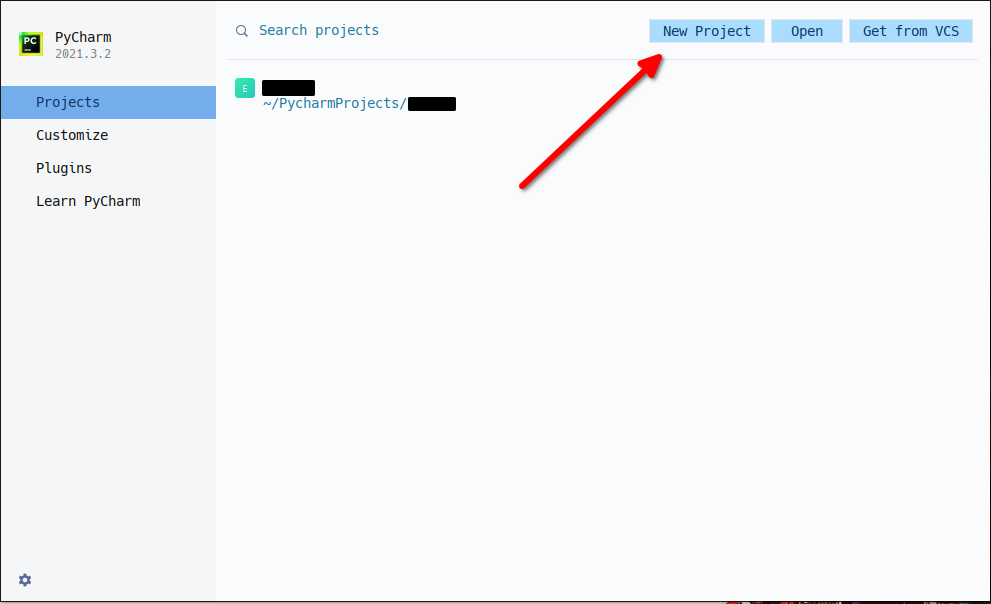
\includegraphics[scale=0.5]{pycharm-new-project.png}
    \end{center}
\end{figure}

\begin{figure}[!ht]
    \begin{center}
        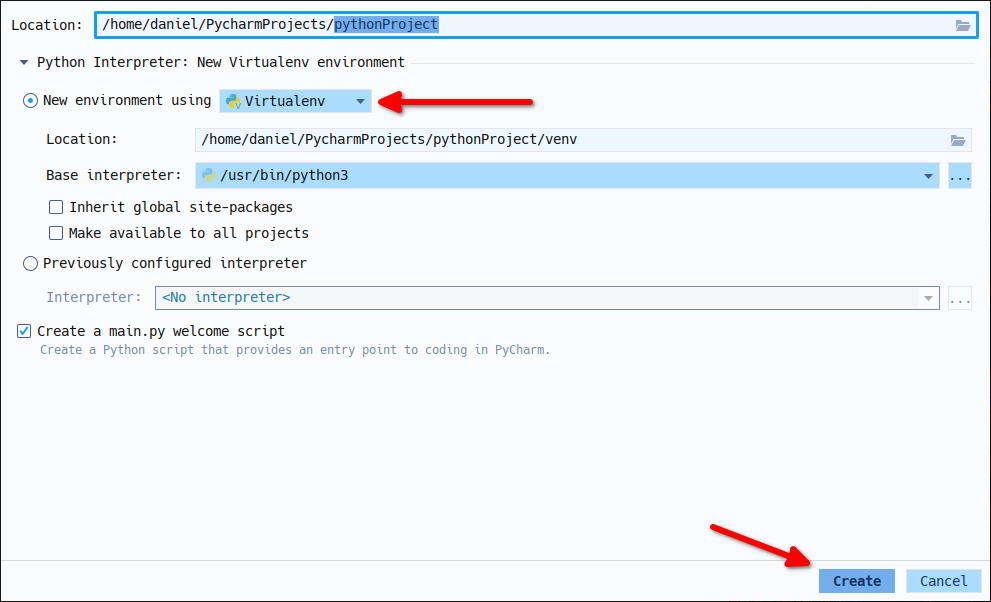
\includegraphics[scale=0.5]{pycharm-create.png}
    \end{center}
\end{figure}

To create a virtual environment without an IDE it is necessary to use the terminal or command line. On windows it can be accessed by pressing WindowsKey + R, and writing "cmd" on the prompt. Clicking "Ok" will then open the terminal.

On Mac, the terminal can be opened by clicking on the Launchpad icon, typing "terminal" and clicking on the Terminal program.

On Linux, I trust you. %jajajajajajajajajaja 

Once the terminal is open, a virtual environment can be created by running the command
\begin{tcolorbox}[
    enhanced,
    attach boxed title to top left={xshift=6mm,yshift=-3mm},
    colback=lightgreen!20,
    colframe=lightgreen,
    colbacktitle=lightgreen,
    sharp corners,
    ]
    \begin{minted}{fish}
python -m venv [directory]
    \end{minted}
\end{tcolorbox}
\noindent where [directory] is the path to the directory in which you will create the environment. After the virtual environment is created, it can be activated by running a script installed by venv. On windows, this is done with
\begin{tcolorbox}[
    enhanced,
    attach boxed title to top left={xshift=6mm,yshift=-3mm},
    colback=lightgreen!20,
    colframe=lightgreen,
    colbacktitle=lightgreen,
    sharp corners,
    ]
    \begin{minted}{text}
myenv\Scripts\activate.bat
    \end{minted}
\end{tcolorbox}
\noindent on either Mac or Linux this is done with
\begin{tcolorbox}[
    enhanced,
    attach boxed title to top left={xshift=6mm,yshift=-3mm},
    colback=lightgreen!20,
    colframe=lightgreen,
    colbacktitle=lightgreen,
    sharp corners,
    ]
    \begin{minted}{text}
source myenv/bin/activate
    \end{minted}
\end{tcolorbox}
\noindent where ``myenv'' is the name of the virtual environment directory just created.

After the environment is activated, any packages that are installed will only be so in the local environment. Python scripts that are run while inside the environment will be able to use any packages installed in it.

To deactivate or exit a virtual environment one only needs to run ``deactivate'' in the terminal. PyCharm automatically opens and closes virtual environments when opening and closing projects.

\subsection{Python basics}

Providing an introductory course to Python is not the purpose of this guide. However, aiming to be as accessible as possible, the very basics needed to understand and use the {\scshape MedPCPy} library will be explained.

\subsubsection{Data types}

Several data types are available in Python. The most common ones are \verb|strings|, \verb|integers|, \verb|floats|, \verb|lists|, \verb|tuples|, \verb|dictionaries|, and \verb|booleans|.

\vspace{5mm}
\noindent\begin{tabular}{|c|c|c|c|}
    \hline
    {\bfseries Name}&{\bfseries Type}&{\bfseries Description}&{\bfseries Examples}\\
    \hline
    Strings&str&Ordered sequence of characters&"Hello, world"\ \ \ "123"\\
    \hline
    Integers&int&Whole numbers&0\ \ \ 399\ \ \ 1996\\
    \hline
    Floating points&float&Numbers with a decimal point&0.0\ \ \ 3.1415\\
    \hline
    Lists&list&Ordered sequence of objects&[1, 3.6, "one"]\\
    \hline
    Tuples&tup&Non-modifiable list&(10, "hello", 1.4)\\
    \hline
    Dictionaries&dict&Ordered Key:Value pairs&\{"name": "Giorno", "age": 15\}\\
    \hline
    Boolean&bool&Logical \verb|True|/\verb|False| values&\verb|True|\ \ \ \verb|False|\\
    \hline
\end{tabular}

\vspace{5mm}
\subsubsection{Variable assignment}

All data types can be assigned to variables to make them more manageable.

\begin{tcolorbox}[
    enhanced,
    attach boxed title to top left={xshift=6mm,yshift=-3mm},
    colback=lightgreen!20,
    colframe=lightgreen,
    colbacktitle=lightgreen,
    title=Python,
    fonttitle=\bfseries\color{black},
    boxed title style={size=small,colframe=lightgreen,sharp corners},
    sharp corners,
    ]
    \begin{minted}[linenos]{python}
my_string = "Hello, world!"
my_int = 745
my_float = 100.0
my_list = [my_string, my_int, my_float]
my_tuple = (my_string, my_int, my_float, my_list)
my_dict = {
    "name": "Joseph",
    "nationality": "english",
    "age": 18
}
my_bool = True
    \end{minted}
\end{tcolorbox}

As you can see, having named variables instead of crude data is more readable. It also allows the use of a previously declared variable on the declaration of another one.

\subsubsection{Nesting}

Lists, tuples, and dictionaries allow nesting other lists, tuples or dictionaries within them with no limit to how deep the nesting can go.

\begin{tcolorbox}[
    enhanced,
    attach boxed title to top left={xshift=6mm,yshift=-3mm},
    colback=lightgreen!20,
    colframe=lightgreen,
    colbacktitle=lightgreen,
    title=Python,
    fonttitle=\bfseries\color{black},
    boxed title style={size=small,colframe=lightgreen,sharp corners},
    sharp corners,
    ]
    \begin{minted}[linenos]{python}
list_1 = [1, 2, 3, 4]
list_2 = [5, 6, 7, 8]
super_list = [list_1, list_2]
    \end{minted}
\end{tcolorbox}

In this example the variable \verb|super_list| would contain two items, both of which would be lists. I.e., the code above is equivalent to:

\begin{tcolorbox}[
    enhanced,
    attach boxed title to top left={xshift=6mm,yshift=-3mm},
    colback=lightgreen!20,
    colframe=lightgreen,
    colbacktitle=lightgreen,
    title=Python,
    fonttitle=\bfseries\color{black},
    boxed title style={size=small,colframe=lightgreen,sharp corners},
    sharp corners,
    ]
    \begin{minted}[linenos]{python}
super_list = [[1, 2, 3, 4], [5, 6, 7, 8]]
    \end{minted}
\end{tcolorbox}

And the same is true for either tuples or dictionaries:

\begin{tcolorbox}[
    enhanced,
    attach boxed title to top left={xshift=6mm,yshift=-3mm},
    colback=lightgreen!20,
    colframe=lightgreen,
    colbacktitle=lightgreen,
    title=Python,
    fonttitle=\bfseries\color{black},
    boxed title style={size=small,colframe=lightgreen,sharp corners},
    sharp corners,
    ]
    \begin{minted}[linenos]{python}
super_tuple = (("a", "b", "c"), "d")
dictionary = {
    "names": ["Jonathan", "Joseph", "Giorno"],
    "nationalities": ["english", "american", "italian"]
}
    \end{minted}
\end{tcolorbox}

This is also not limited to the same type of variable. That is, lists can contain tuples and dictionaries, tuples can contain lists and dictionaries, and so on.

Dictionaries can even be nested inside other dictionaries:

\begin{tcolorbox}[
    enhanced,
    attach boxed title to top left={xshift=6mm,yshift=-3mm},
    colback=lightgreen!20,
    colframe=lightgreen,
    colbacktitle=lightgreen,
    title=Python,
    fonttitle=\bfseries\color{black},
    boxed title style={size=small,colframe=lightgreen,sharp corners},
    sharp corners,
    ]
    \begin{minted}[linenos]{python}
planets = {
    "earth": {"color": "blue", "population": "lots"},
    "mars": {"color": "red", "population": "none"}
}
    \end{minted}
\end{tcolorbox}

The analysis list used in the {\scshape MedPCPy} library is a list comprised of dictionaries with other, nested dictionaries:

\begin{tcolorbox}[
    enhanced,
    attach boxed title to top left={xshift=6mm,yshift=-3mm},
    colback=lightgreen!20,
    colframe=lightgreen,
    colbacktitle=lightgreen,
    title=Python,
    fonttitle=\bfseries\color{black},
    boxed title style={size=small,colframe=lightgreen,sharp corners},
    sharp corners,
    ]
    \begin{minted}[linenos]{python}
analysis_list = [
    # Measure 1
    {"fetch": {"cell_row": 1,
               "cell_column": 1,
               "sheet": "Measure1",
               "summary_column_dict": measure1_cols,
               "offset": 0,
               }},
               ...
                ]
    \end{minted}
\end{tcolorbox}

Be mindful that the use of space in the declaration of lists, tuples or dictionaries has no syntactic purpose. The distribution is only to increase readability.

\subsubsection{Functions}

Functions are blocks of reusable code which perform actions that are needed frequently. They are declared only once, and after that they are executed when called. They help increase the readability and modularity of code. %"They are declared only once, but can be executed everytime the are called".

Functions are declared with the \verb|def| keyword, followed by the function name, optionally the arguments in parentheses, and a semicolon. They can either only perform an action, or return a value which can then be assigned to a variable.

\begin{tcolorbox}[
    enhanced,
    attach boxed title to top left={xshift=6mm,yshift=-3mm},
    colback=lightgreen!20,
    colframe=lightgreen,
    colbacktitle=lightgreen,
    title=Python,
    fonttitle=\bfseries\color{black},
    boxed title style={size=small,colframe=lightgreen,sharp corners},
    sharp corners,
    ]
    \begin{minted}[linenos]{python}
def hello_function():
    print("Pizza Mozzarella")

def my_sum_function(a, b):
    return a + b
    \end{minted}
\end{tcolorbox}

Then they are called with their name and the necessary arguments:

\begin{tcolorbox}[
    enhanced,
    attach boxed title to top left={xshift=6mm,yshift=-3mm},
    colback=lightgreen!20,
    colframe=lightgreen,
    colbacktitle=lightgreen,
    title=Python,
    fonttitle=\bfseries\color{black},
    boxed title style={size=small,colframe=lightgreen,sharp corners},
    sharp corners,
    ]
    \begin{minted}[linenos]{python}
hello_function()

x = 20
y = 30
result = my_sum_function(x, y)
    \end{minted}
\end{tcolorbox}

This would result in the string \verb|"Pizza Mozzarella"| being printed, and the number \verb|50| being assigned to the variable \verb|result|. %No sé si aquí sirva tener el resultado visible, yo lo entiendo pero no sé si alguien muy nuevo entienda por qué sale. 

Functions can have positional arguments (identified by their position) and keyword arguments (identified by a keyword). Additionally, if a default value for an argument is provided when the function is defined, then that argument becomes optional and, if it is not declared when the function is called, it will take the default value.

\begin{tcolorbox}[
    enhanced,
    attach boxed title to top left={xshift=6mm,yshift=-3mm},
    colback=lightgreen!20,
    colframe=lightgreen,
    colbacktitle=lightgreen,
    title=Python,
    fonttitle=\bfseries\color{black},
    boxed title style={size=small,colframe=lightgreen,sharp corners},
    sharp corners,
    ]
    \begin{minted}[linenos]{python}
def another_function(name = "Ford Prefect"):
    print(f"Hello, my name is {name}")

another_function()
    \end{minted}
\end{tcolorbox}

This would print the string \verb|"Hello, my name is Ford Prefect"|, since the optional argument \verb|name| took the default value \verb|Ford Prefect|. %Este ejemplo sí me parece más "claro" aunque no sepas de programación.

\subsubsection{Classes and objects}

Python is an object-oriented programming language, which means that a good deal of its functionality is built around ``objects'' which contain data and code. In object-oriented programming the code is organized into reusable ``blueprints'' called \verb|classes|, and those classes can be used to create individual instances of \verb|objects|. Objects have properties (data) and methods (functions) associated to them.

A class is declared with the \verb|class| keyword, the name of the class, and a semicolon. Class attributes are declared in a special function called \verb|__init__|, and methods associated with the class are declared as functions inside of it.

\begin{tcolorbox}[
    enhanced,
    attach boxed title to top left={xshift=6mm,yshift=-3mm},
    colback=lightgreen!20,
    colframe=lightgreen,
    colbacktitle=lightgreen,
    title=Python,
    fonttitle=\bfseries\color{black},
    boxed title style={size=small,colframe=lightgreen,sharp corners},
    sharp corners,
    ]
    \begin{minted}[linenos]{python}
class Dog:
    def __init__(name, age):
        self.dog_name = name
        self.dog_age = age

    def print_name():
        print(f"""
        Hello, my name is {self.dog_name},
        and I am {self.dog_age} years old. Woof!
        """)
    \end{minted}
\end{tcolorbox}

Afterwards, the class can be used as a blueprint to create individual objects with the general properties of the class.

\begin{tcolorbox}[
    enhanced,
    attach boxed title to top left={xshift=6mm,yshift=-3mm},
    colback=lightgreen!20,
    colframe=lightgreen,
    colbacktitle=lightgreen,
    title=Python,
    fonttitle=\bfseries\color{black},
    boxed title style={size=small,colframe=lightgreen,sharp corners},
    sharp corners,
    ]
    \begin{minted}[linenos]{python}
my_dog = Dog("John", 5)
    \end{minted}
\end{tcolorbox}

The creation of the object is similar to the calling of a function. In this example the end result would be an object of class \verb|Dog| being assigned to the variable \verb|my_dog|. This object would have two attributes and a method associated. The attributes can be changed with the notation \verb|object.attribute = [new value]|.

\begin{tcolorbox}[
    enhanced,
    attach boxed title to top left={xshift=6mm,yshift=-3mm},
    colback=lightgreen!20,
    colframe=lightgreen,
    colbacktitle=lightgreen,
    title=Python,
    fonttitle=\bfseries\color{black},
    boxed title style={size=small,colframe=lightgreen,sharp corners},
    sharp corners,
    ]
    \begin{minted}[linenos]{python}
my_dog.dog_name = "Tovarisch" %Dados los eventos recientes, no sé si sea buena idea usar la palabra Tovarisch :(
    \end{minted}
\end{tcolorbox}

And the method can be used with the notation \verb|object.method()|.

\begin{tcolorbox}[
    enhanced,
    attach boxed title to top left={xshift=6mm,yshift=-3mm},
    colback=lightgreen!20,
    colframe=lightgreen,
    colbacktitle=lightgreen,
    title=Python,
    fonttitle=\bfseries\color{black},
    boxed title style={size=small,colframe=lightgreen,sharp corners},
    sharp corners,
    ]
    \begin{minted}[linenos]{python}
my_dog.print_name()
    \end{minted}
\end{tcolorbox}

This would result in printing the phrase

\begin{tcolorbox}[
    enhanced,
    attach boxed title to top left={xshift=6mm,yshift=-3mm},
    colback=lightgray!20,
    colframe=lightgray,
    colbacktitle=lightgreen,
    sharp corners,
    ]
    \begin{minted}{text}
Hello, my name is Tovarisch,
and I am 5 years old. Woof!
    \end{minted}
\end{tcolorbox}

\newpage
\section{This library}




\end{document}
